\documentclass[tikz,border=10pt]{standalone}
\usetikzlibrary{shapes.multipart, positioning, arrows.meta}

\begin{document}
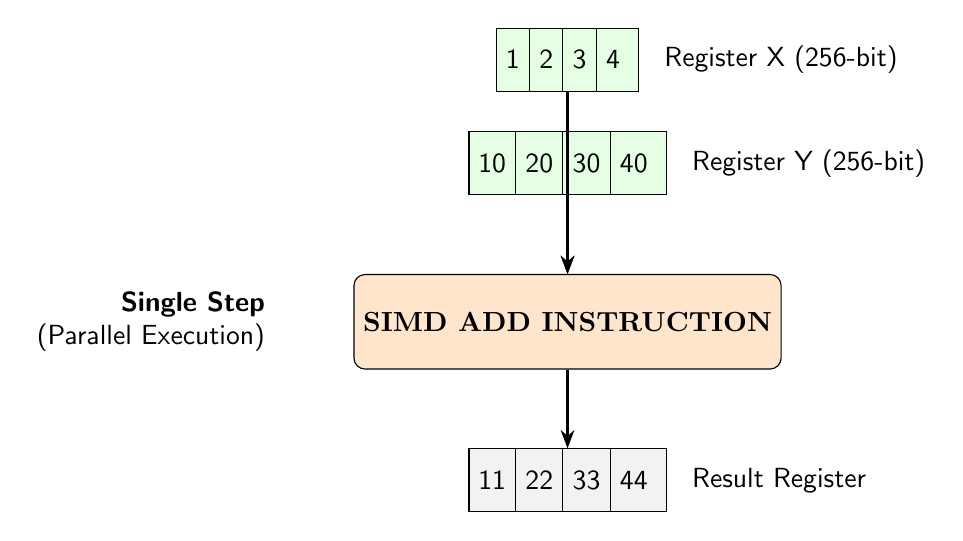
\begin{tikzpicture}[
    node distance=1.0cm,
    font=\sffamily,
    % Styles
    vector/.style={
        draw,
        rectangle split,
        rectangle split parts=4,
        rectangle split horizontal,
        minimum height=0.8cm,
        align=center,
        fill=green!10
    },
    simd_op/.style={
        draw,
        rounded corners,
        fill=orange!20,
        minimum width=5cm,
        minimum height=1.2cm,
        align=center,
        font=\bfseries
    },
    arrow/.style={->, >=Stealth, thick}
]

    % --- INPUT VECTORS ---
    % Vector X
    \node[vector] (vx) {
        \nodepart{one} 1
        \nodepart{two} 2
        \nodepart{three} 3
        \nodepart{four} 4
    };
    \node[right=0.2cm of vx] {Register X (256-bit)};

    % Vector Y
    \node[vector, below=0.5cm of vx] (vy) {
        \nodepart{one} 10
        \nodepart{two} 20
        \nodepart{three} 30
        \nodepart{four} 40
    };
    \node[right=0.2cm of vy] {Register Y (256-bit)};

    % --- SIMD OPERATION ---
    \node[simd_op, below=1cm of vy] (alu) {SIMD ADD INSTRUCTION};

    % --- RESULT VECTOR ---
    \node[vector, fill=gray!10, below=1cm of alu] (vres) {
        \nodepart{one} 11
        \nodepart{two} 22
        \nodepart{three} 33
        \nodepart{four} 44
    };
    \node[right=0.2cm of vres] {Result Register};

    % --- ARROWS ---
    % We use coordinate calculations to draw clean arrows from the centers
    \draw[arrow] (vx) -- (vx|-alu.north);
    \draw[arrow] (vy) -- (alu);
    \draw[arrow] (alu) -- (vres);

    % Annotation
    \node[left=1cm of alu, align=right] {\textbf{Single Step}\\(Parallel Execution)};

\end{tikzpicture}
\end{document}
